\documentclass[tikz, convert = false]{standalone}%

\usepackage[utf8]{inputenx}%  http://ctan.org/pkg/inputenx
% Euler for math | Palatino for rm | Helvetica for ss | Courier for tt
\renewcommand{\rmdefault}{ppl}% rm
\linespread{1.05}% Palatino needs more leading
\usepackage[scaled]{helvet}% ss //  http://ctan.org/pkg/helvet
\usepackage{courier}% tt // http://ctan.org/pkg/courier
\usepackage{eulervm}  %  http://ctan.org/pkg/eulervm
% a better implementation of the euler package (not in gwTeX)
\normalfont%
\usepackage[T1]{fontenc}%  http://ctan.org/pkg/fontenc
\usepackage{textcomp}%  http://ctan.org/pkg/textcomp

\usetikzlibrary{calc}
\usetikzlibrary{intersections}
\usetikzlibrary{backgrounds}

\begin{document}
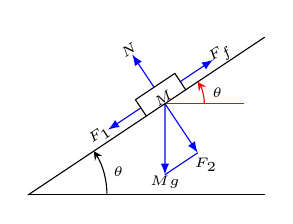
\begin{tikzpicture}[line join = round, line cap = round]
  \coordinate (O) at (0, 0);

  \draw (O) -- +(3, 0) coordinate (P1);
  \draw[name path = sline] (O) -- (3, 2) coordinate (P2);

  \draw[-stealth] let
    \p0 = (O),
    \p1 = (P1),
    \p2 = (P2),
    \n1 = {atan2(\y1 - \y0, \x1 - \x0)},
    \n2 = {atan2(\y2 - \y0, \x2 - \x0)},
    \n3 = {1cm},
    \n4 = {(\n1 + \n2)/2}
  in \pgfextra{\xdef\myn{\n2}} (O) +(\n1:\n3) arc[radius = \n3,
  start angle = \n1, end angle = \n2] node[right, font = \tiny] at (\n4:\n3)
  {$\theta$};

  \path[name path = line1] (1.5, 0) -- +(0, 1.25);
  \path[name path = line2] (2, 0) -- +(0, 1.5);
  \path[name intersections = {of = sline and line1, by = P3}];
  \path[name intersections = {of = sline and line2, by = P4}];
  
  \draw (P3) -- ($(P3)!.25cm!-90:(O)$) coordinate (P5);
  \draw (P4) -- ($(P4)!.25cm!-90:(O)$) coordinate (P6);
  \draw[name path = boxtop] (P5) -- (P6) node[pos = .5, below, font = \tiny,
  rotate = \myn] {$M$};

  \path[name path = grav] ($(P5)!.75!(P6)$) -- +(0, -1.25);
  \path[name intersections = {of = grav and sline, by = P7}];
  
  \begin{scope}[on background layer]
    \draw[-latex, blue] (P7) -- ($(P7)!.75cm!-270:(O)$) coordinate (P8)
    node[pos = 1.25, font = \tiny, color = black] {$F_2$};

    \path[name path = perl1] (P8) -- ($(P8)!.75cm!-270:(P7)$);
    \path[name intersections = {of = perl1 and grav, by = P9}];
    
    \draw[-latex, blue] (P7) -- (P9) node[below, font = \tiny, inner sep = .3,
    color = black] {$Mg$};
    \draw[blue] (P9) -- (P8);

    \path[name path = norm] (P7) -- ($(P7)!.75cm!-90:(O)$);
    \path[name intersections = {of = norm and boxtop, by = P10}];

    \draw[-latex,blue] (P10) -- ($(P10)!.5cm!-90:(P5)$) node[pos = 1.15,
    font = \tiny, rotate = {\myn}, color = black] {$N$};

    \coordinate (P11) at ($(P3)!.5!(P5)$);
    \coordinate (P12) at ($(P4)!.5!(P6)$);

    \draw[-latex, blue] (P12) -- ++(\myn:.5) node[pos = 1.25, font = \tiny,
    rotate = {\myn}, color = black] {$F_f$};
    \draw[-latex, blue] (P11) -- ++({\myn + 180}:.5) node[pos = 1.25,
    font = \tiny, rotate = {\myn}, color = black] {$F_1$};
    \draw[red] (P7) -- +(1, 0) coordinate (P13);

    \draw[-stealth, red] let
      \p0 = (P7),
      \p1 = (P2),
      \p2 = (P13),
      \n1 = {atan2(\y2 - \y0, \x2 - \x0)},
      \n2 = {atan2(\y1 - \y0, \x1 - \x0)},
      \n3 = {.5cm},
      \n4 = {(\n1 + \n2)/2}
    in (P7) +(\n1:\n3) arc[radius = \n3, start angle = \n1, end angle = \n2]
    node[font = \tiny, right, color = black] at ([shift = (P7)] \n4:\n3)
    {$\theta$};
  \end{scope}
\end{tikzpicture}
\end{document}
%%% Local Variables:
%%% mode: latex
%%% TeX-master: t
%%% End:
